%%% The main file. It contains definitions of basic parameters and includes all other parts.

%% Settings for single-side (simplex) printing
% Margins: left 40mm, right 25mm, top and bottom 25mm
% (but beware, LaTeX adds 1in implicitly)
\documentclass[12pt,a4paper]{report}
\setlength\textwidth{145mm}
\setlength\textheight{247mm}
\setlength\oddsidemargin{15mm}
\setlength\evensidemargin{15mm}
\setlength\topmargin{0mm}
\setlength\headsep{0mm}
\setlength\headheight{0mm}
% \openright makes the following text appear on a right-hand page
\let\openright=\clearpage

%% Settings for two-sided (duplex) printing
% \documentclass[12pt,a4paper,twoside,openright]{report}
% \setlength\textwidth{145mm}
% \setlength\textheight{247mm}
% \setlength\oddsidemargin{14.2mm}
% \setlength\evensidemargin{0mm}
% \setlength\topmargin{0mm}
% \setlength\headsep{0mm}
% \setlength\headheight{0mm}
% \let\openright=\cleardoublepage

%% Generate PDF/A-2u
\usepackage[a-2u]{pdfx}

%% Character encoding: usually latin2, cp1250 or utf8:
\usepackage[utf8]{inputenc}

%% Prefer Latin Modern fonts
\usepackage{lmodern}

%% Further useful packages (included in most LaTeX distributions)
\usepackage{amsmath}        % extensions for typesetting of math
\usepackage{amsfonts}       % math fonts
\usepackage{amsthm}         % theorems, definitions, etc.
\usepackage{bbding}         % various symbols (squares, asterisks, scissors, ...)
\usepackage{bm}             % boldface symbols (\bm)
\usepackage{graphicx}       % embedding of pictures
\usepackage{fancyvrb}       % improved verbatim environment
\usepackage{natbib}         % citation style AUTHOR (YEAR), or AUTHOR [NUMBER]
\usepackage[nottoc]{tocbibind} % makes sure that bibliography and the lists
			    % of figures/tables are included in the table
			    % of contents
\usepackage{dcolumn}        % improved alignment of table columns
\usepackage{booktabs}       % improved horizontal lines in tables
\usepackage{paralist}       % improved enumerate and itemize
\usepackage{xcolor}         % typesetting in color
\usepackage{enumitem}

%%% Basic information on the thesis

% Thesis title in English (exactly as in the formal assignment)
\def\ThesisTitle{Dietary profile and customized menus using Solid}

% Author of the thesis
\def\ThesisAuthor{Bc. Jiří Resler}

% Year when the thesis is submitted
\def\YearSubmitted{2023}

% Name of the department or institute, where the work was officially assigned
% (according to the Organizational Structure of MFF UK in English,
% or a full name of a department outside MFF)
\def\Department{Department of Software Engineering}

% Is it a department (katedra), or an institute (ústav)?
\def\DeptType{Department}

% Thesis supervisor: name, surname and titles
\def\Supervisor{RNDr. Jakub Klímek, Ph.D.}

% Supervisor's department (again according to Organizational structure of MFF)
\def\SupervisorsDepartment{Department of Software Engineering}

% Study programme and specialization
\def\StudyProgramme{Software and Data Engineering}
\def\StudyBranch{Software engineering}

% An optional dedication: you can thank whomever you wish (your supervisor,
% consultant, a person who lent the software, etc.)
\def\Dedication{%
Dedication.
}

% Abstract (recommended length around 80-200 words; this is not a copy of your thesis assignment!)
\def\Abstract{%
Abstract.
}

% 3 to 5 keywords (recommended), each enclosed in curly braces
\def\Keywords{%
{solid}, {data}, {linked data}, {RDF}, {redecentralization of web}, {read write web}, {diet}, {food}
}

%% The hyperref package for clickable links in PDF and also for storing
%% metadata to PDF (including the table of contents).
%% Most settings are pre-set by the pdfx package.
\hypersetup{unicode}
\hypersetup{breaklinks=true}

% Definitions of macros (see description inside)
%%% This file contains definitions of various useful macros and environments %%%
%%% Please add more macros here instead of cluttering other files with them. %%%

%%% Minor tweaks of style

% These macros employ a little dirty trick to convince LaTeX to typeset
% chapter headings sanely, without lots of empty space above them.
% Feel free to ignore.
\makeatletter
\def\@makechapterhead#1{
  {\parindent \z@ \raggedright \normalfont
   \Huge\bfseries \thechapter. #1
   \par\nobreak
   \vskip 20\p@
}}
\def\@makeschapterhead#1{
  {\parindent \z@ \raggedright \normalfont
   \Huge\bfseries #1
   \par\nobreak
   \vskip 20\p@
}}
\makeatother

% This macro defines a chapter, which is not numbered, but is included
% in the table of contents.
\def\chapwithtoc#1{
\chapter*{#1}
\addcontentsline{toc}{chapter}{#1}
}

% Draw black "slugs" whenever a line overflows, so that we can spot it easily.
\overfullrule=1mm

%%% Macros for definitions, theorems, claims, examples, ... (requires amsthm package)

\theoremstyle{plain}
\newtheorem{thm}{Theorem}
\newtheorem{lemma}[thm]{Lemma}
\newtheorem{claim}[thm]{Claim}

\theoremstyle{plain}
\newtheorem{defn}{Definition}

\theoremstyle{remark}
\newtheorem*{cor}{Corollary}
\newtheorem*{rem}{Remark}
\newtheorem*{example}{Example}

%%% An environment for proofs

\newenvironment{myproof}{
  \par\medskip\noindent
  \textit{Proof}.
}{
\newline
\rightline{$\qedsymbol$}
}

%%% An environment for typesetting of program code and input/output
%%% of programs. (Requires the fancyvrb package -- fancy verbatim.)

\DefineVerbatimEnvironment{code}{Verbatim}{fontsize=\small, frame=single}

%%% The field of all real and natural numbers
\newcommand{\R}{\mathbb{R}}
\newcommand{\N}{\mathbb{N}}

%%% Useful operators for statistics and probability
\DeclareMathOperator{\pr}{\textsf{P}}
\DeclareMathOperator{\E}{\textsf{E}\,}
\DeclareMathOperator{\var}{\textrm{var}}
\DeclareMathOperator{\sd}{\textrm{sd}}

%%% Transposition of a vector/matrix
\newcommand{\T}[1]{#1^\top}

%%% Various math goodies
\newcommand{\goto}{\rightarrow}
\newcommand{\gotop}{\stackrel{P}{\longrightarrow}}
\newcommand{\maon}[1]{o(n^{#1})}
\newcommand{\abs}[1]{\left|{#1}\right|}
\newcommand{\dint}{\int_0^\tau\!\!\int_0^\tau}
\newcommand{\isqr}[1]{\frac{1}{\sqrt{#1}}}

%%% Various table goodies
\newcommand{\pulrad}[1]{\raisebox{1.5ex}[0pt]{#1}}
\newcommand{\mc}[1]{\multicolumn{1}{c}{#1}}


% Title page and various mandatory informational pages
\begin{document}
%%% Title page of the thesis and other mandatory pages

%%% Title page of the thesis

\pagestyle{empty}
\hypersetup{pageanchor=false}
\begin{center}

\centerline{\mbox{
\includegraphics[width=166mm]{../img/logo-en.pdf}}}

\vspace{-8mm}
\vfill

{\bf\Large MASTER THESIS}

\vfill

{\LARGE\ThesisAuthor}

\vspace{15mm}

{\LARGE\bfseries\ThesisTitle}

\vfill

\Department

\vfill

{
\centerline{\vbox{\halign{\hbox to 0.45\hsize{\hfil #}&\hskip 0.5em\parbox[t]{0.45\hsize}{\raggedright #}\cr
Supervisor of the master thesis:&\Supervisor \cr
\noalign{\vspace{2mm}}
Study programme:&\StudyProgramme \cr
\noalign{\vspace{2mm}}
Study branch:&\StudyBranch \cr
}}}}

\vfill

% Zde doplňte rok
Prague \YearSubmitted

\end{center}

\newpage

%%% Here should be a bound sheet included -- a signed copy of the "master
%%% thesis assignment". This assignment is NOT a part of the electronic
%%% version of the thesis. DO NOT SCAN.

%%% A page with a solemn declaration to the master thesis

\openright
\hypersetup{pageanchor=true}
\pagestyle{plain}
\pagenumbering{roman}
\vglue 0pt plus 1fill

\noindent
I declare that I carried out this master thesis independently, and only with the cited
sources, literature and other professional sources. It has not been used to obtain another
or the same degree.

\medskip\noindent
I understand that my work relates to the rights and obligations under the Act No.~121/2000 Sb.,
the Copyright Act, as amended, in particular the fact that the Charles
University has the right to conclude a license agreement on the use of this
work as a school work pursuant to Section 60 subsection 1 of the Copyright~Act.

\vspace{10mm}

\hbox{\hbox to 0.5\hsize{%
In \hbox to 6em{\dotfill} date \hbox to 6em{\dotfill}
\hss}\hbox to 0.5\hsize{\dotfill\quad}}
\smallskip
\hbox{\hbox to 0.5\hsize{}\hbox to 0.5\hsize{\hfil Author's signature\hfil}}

\vspace{20mm}
\newpage

%%% Dedication

\openright

\noindent
\Dedication

\newpage

%%% Mandatory information page of the thesis

\openright

\vbox to 0.5\vsize{
\setlength\parindent{0mm}
\setlength\parskip{5mm}

Title:
\ThesisTitle

Author:
\ThesisAuthor

\DeptType:
\Department

Supervisor:
\Supervisor, \SupervisorsDepartment

Abstract:
\Abstract

Keywords:
\Keywords

\vss}

\newpage

\openright
\pagestyle{plain}
\pagenumbering{arabic}
\setcounter{page}{1}


%%% A page with automatically generated table of contents of the master thesis

\tableofcontents

%%% Each chapter is kept in a separate file
\chapter*{Introduction}
\addcontentsline{toc}{chapter}{Introduction}

Health is the most important thing we have in our lives.
If we want to be healthy we need to, among other things, think about what we eat.
People today are trying various diets in order to stay in shape and feel good.
There are also many people who suffer from food allergies who need to pick carefully what they eat, as some food is harmful to them. 

If a person who is on a diet or has an allergy decides to visit a restaurant which they have never been to, they spend a lot of time reading the restaurant's menu. 
They need to browse it and read ingredients of every meal in order to find one which is healthy for them to eat.

In this thesis we will document the process of the creation of a web application whose purpose will be to help these people to be able to quickly choose what they want to eat at a restaurant. 
The application will achieve this by letting its users create their personal profile and within it to specify what allergies they have or what diets they are on. 
It will also enable restaurant providers to create menus online. 
When a visitor will browse a restaurant's menu, the application will make it possible to only display those meals which the visitor is able to eat according to their profile.

Also, we need to be aware that whether someone is on a diet or has an allergy are personal information which the user may be sensitive about.

We will therefor design and implement the application in a safe and modern way which will ensure that only the user can view and manipulate with their personal profile data.


\chapter{Preliminaries}
We will start by introducing the Solid technology.
This chapter contains an explanation of terms specific to Solid which will be used throughout this thesis.

% Glossary
% EU - European Union
% Solid

% Solid pod

% WebID

% IRI

% URL

% Solid provider

% \section{Semantic Web - the Solid technology}

\chapter{Problem analysis}
Our first step will be to define what will the application do and also who will be able to use it.
For this reason we will identify user roles, specify use cases and describe those via use case scenarios.
The output of this chapter is a list of user requirements which will be important in the next chapter.
This analysis is inspired by interviewing a restaurant\footnote{\url{https://www.pizzabudca.sk}  \label{fnlabel}} employee and also two former restaurant\footnote{\url{https://www.sokolzabreh.cz/hospudka}  \label{fnlabel}} owners.

\section{Target group}
The application will focus on restaurants and their guests in the European Union.
The reason behind this is that the EU enforces restaurants to inform their guests about allergens contained in the food they serve, and has already established rules for how to do it.
We would like for the application to be usable internationally, so it needs to have its user interface translated into different languages.
For this purpose we will choose the English, Slovak and Czech languages with the possibility of adding more translations in the future.

\section{User roles}
There are two types of users who will come in contact with the application.
The first type is a \textbf{restaurant}, more specifically its employee who is responsible for creating menus.
This user needs to have a basic understanding of how to use a web browser either on a computer or on a smartphone.
The application will allow restaurant employees to create menus online and will help them with specifying allergens contained in menu items.

The second type of user is a restaurant \textbf{guest}.
They, too, need to have a basic understanding of how to use a web browser either on a computer or on a smartphone.
The application will enable a restaurant guest to create a personal profile where they will specify their food preferences, including the allergies they have and the diets they are on.
When a guest will view a restaurant's menu using the application, the displayed menu will be adapted to meet the guest's profile preferences.
The application will thus make it easier for the guest to choose what they would like to order in a particular restaurant.

\newpage

\section{Use cases}
Now we are going to depict goals of users which the application will make achievable.
Figure 2.1 contains a use case diagram of the application.
A use case styled with a bold border groups together more use cases and will be expanded further.
All use cases will be structurally described by independent use case scenarios.
A structured use case will contain a description if the goal of a user is not entirely clear from the use case's name.

\begin{figure}[h]
  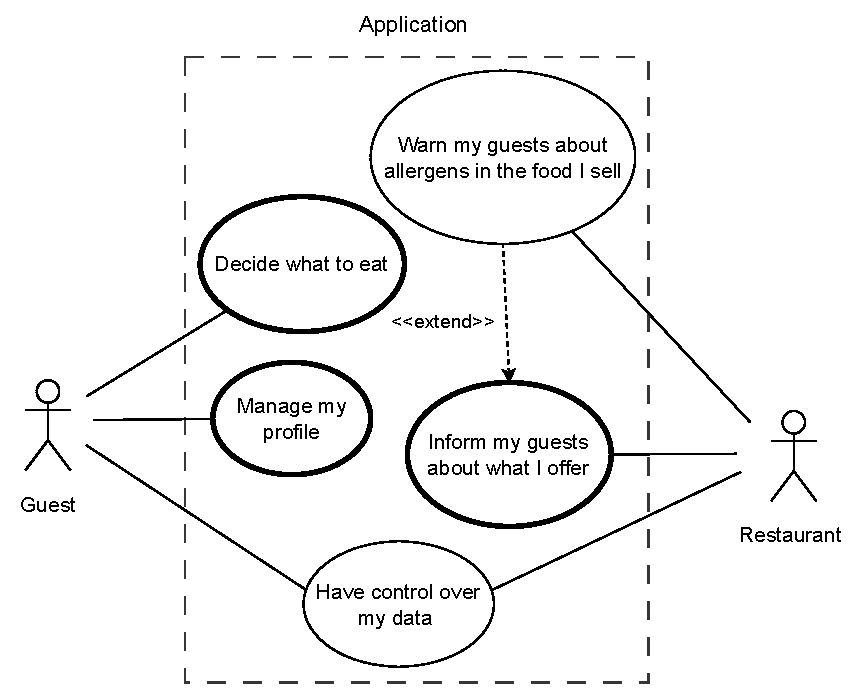
\includegraphics[width=\linewidth]{master-thesis/img/use_cases/use_cases}
  \caption{The application's use case diagram.}
\end{figure}

\newpage

% Add top padding for scenario tables
\def\arraystretch{1.5}

\subsection{Guest use cases}

\begin{figure}[h]
  \centering
  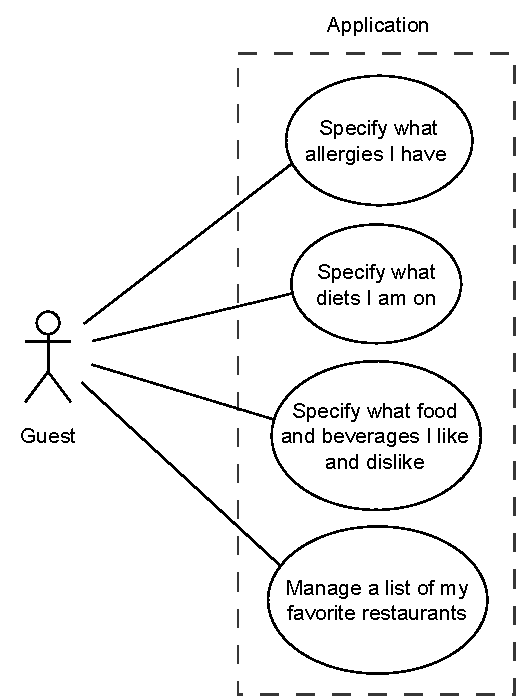
\includegraphics[width=0.62\linewidth]{master-thesis/img/use_cases/use_cases_guest_profile_management}
  \caption{Guest profile management use cases}
\end{figure}

\newpage

\noindent \textbf{1. Use case: Specify what allergies I have}
\begin{center}
  \begin{tabular}{| l | p{10.75cm} | }
    \hline
    Actor       & Guest \\
    \hline
    Description & A guest has a set of allergies which is stored on their Solid pod. The scenario describes how the guest can add allergies to this set and also how the application displays the set. \\
    \hline
    Scenario    &
    \begin{minipage}[t]{\linewidth}
      \begin{enumerate}[leftmargin=*,nosep,before=\vspace{-0.575\baselineskip},after=\strut]
        \item The guest opens their profile.
        \item The guest presses a menu button in the top-left corner of the screen.
        \item The application displays a dropdown list containing links for navigation.
        \item The guest follows a link which says "My allergies".
        \item The application displays a screen with a list of previously specified allergies by the guest. \textbf{A1}
        \item The guest presses a button labeled as "Add allergy".
        \item The application displays a search bar with a placeholder which says "Allergy name".
        \item The guest starts typing the name of an allergy into the search bar.
        \item The application suggests allergies which contain the given input in their name.
        \item The guest selects the desired allergy and presses an "Add" button. \textbf{A2}
        \item The application adds the specified allergy to the set of the guest's allergies and also to the list on the screen. \textbf{A3}
        \item The guest repeats steps 6 to 11 until they have specified all of the food allergies they suffer from.
      \end{enumerate}
    \end{minipage}
    \\
    \hline
    Alternatives &
    \begin{minipage}[t]{\linewidth}
      \begin{description}[nosep,after=\strut]
        \item [A1:] The list is empty because the guest has not specified any allergies yet. The application displays a text containing this information.
        \item [A2:] The application does not recognize the allergy which the guest is trying to add. The guest creates a public issue in the application's repository with a request to add the desired allergy to the application.
        \item [A3:] The allergy the guest has specified is already contained in the set and in the list. The application informs the guest about this fact and the set and the list are not altered.
      \end{description}
    \end{minipage}
    \\
    \hline
  \end{tabular}
  \newline
\end{center}

\newpage

\noindent \textbf{2. Use case: Specify what diets I am on}
\begin{center}
  \begin{tabular}{| l | p{10.75cm} | }
    \hline
    Actor       & Guest \\
    \hline
    Description & A guest has a set of diets which is stored on their Solid pod. The scenario describes how the guest can add diets to this set and also how the application displays the set. \\
    \hline
    Scenario    &
    \begin{minipage}[t]{\linewidth}
      \begin{enumerate}[leftmargin=*,nosep,before=\vspace{-0.575\baselineskip},after=\strut]
        \item The guest opens their profile.
        \item The guest presses a menu button in the top-left corner of the screen.
        \item The application displays a dropdown list containing links for navigation.
        \item The guest follows a link which says "My diets".
        \item The application displays a screen with a list of previously specified diets by the guest. \textbf{A1}
        \item The guest presses a button labeled as "Add diet".
        \item The application displays a search bar with a placeholder which says "Diet name".
        \item The guest starts typing the name of a diet into the search bar.
        \item The application suggests diets which contain the given input in their name.
        \item The guest selects the desired diet and presses an "Add" button. \textbf{A2}
        \item The application adds the specified diet to the set of the guest's diets and also to the list on the screen. \textbf{A3}
        \item The guest repeats steps 6 to 11 until they have specified all of the diets they are on.
      \end{enumerate}
    \end{minipage}
    \\
    \hline
    Alternatives &
    \begin{minipage}[t]{\linewidth}
      \begin{description}[nosep,after=\strut]
        \item [A1:] The list is empty because the guest has not specified any diets yet. The application displays a text containing this information.
        \item [A2:] The application does not recognize the diet which the guest is trying to add. The guest creates a public issue in the application's repository with a request to add the desired diet to the application.
        \item [A3:] The diet the guest has specified is already contained in the set and in the list. The application informs the guest about this fact and the set and the list are not altered.
      \end{description}
    \end{minipage}
    \\
    \hline
  \end{tabular}
  \newline
\end{center}

\newpage

\noindent \textbf{3. Use case: Specify what food and beverages I like and dislike}
\begin{center}
  \begin{tabular}{| l | p{10.75cm} | }
    \hline
    Actor    & Guest \\
    \hline
    Scenario &
    \begin{minipage}[t]{\linewidth}
      \begin{enumerate}[leftmargin=*,nosep,before=\vspace{-0.575\baselineskip},after=\strut]
        \item The guest opens their profile.
        \item The guest selects a tab named "My food preferences".
        \item The application displays two lists, one containing the foods which the guest likes and the other containing the foods which the guest dislikes. \textbf{A1}
        \item The guest clicks a button labeled as "Add food I like". \textbf{A2}
        \item The application provides a search bar with a text saying "Search for a food...".
        \item The guest starts typing the name of the food which they want to add.
        \item The application suggests foods which contain the given input text in their name.
        \item The guest selects the desired food and clicks an "Add" button. \textbf{A3}
        \item The application adds the selected food to the guest's set of foods which they like. \textbf{A4}
      \end{enumerate}
    \end{minipage}
    \\
    \hline
    Alternatives &
    \begin{minipage}[t]{\linewidth}
      \begin{description}[nosep,after=\strut]
        \item [A1:] Either one or both of the lists are empty because the guest has not specified any of their preferred or disliked foods yet. Instead of displaying a list, the application displays a text saying "No food specified".
        \item [A2:] The guest clicks a button labeled as "Add food I dislike". The scenario continues with a difference that in the step number 9, the application adds the food to the guest's set of foods which they \emph{dislike}.
        \item [A3:] The application does not recognize the food which the guest is searching for. The guest creates an issue in the application's public repository with a request to add the desired food to the application.
        \item [A4:] The set already contains the food. The guest is informed about this fact and the set is not altered.
      \end{description}
    \end{minipage}
    \\
    \hline
  \end{tabular}
  \newline
\end{center}

\newpage

\noindent \textbf{4. Use case: Manage a list of my favorite restaurants}

\begin{center}
  \begin{tabular}{| l | p{10.75cm} | }
    \hline
    Actor    & Guest \\
    \hline
    Description & A guest has a set of their favorite restaurants which is stored on their Solid pod. The scenario describes how the guest can add or remove a restaurant from this set and how the application displays the set. \\
    \hline
    Scenario &
    \begin{minipage}[t]{\linewidth}
      \begin{enumerate}[leftmargin=*,nosep,before=\vspace{-0.575\baselineskip},after=\strut]
        \item The guest opens their profile. \textbf{A1}
        \item The guest presses a menu button in the top-left corner of the screen.
        \item The application displays a dropdown list containing links for navigation.
        \item The guest follows a link which says "My favorite restaurants".
        \item The application displays a screen with a list containing the guest's favorite restaurants. \textbf{A2} 
        \item The guest presses an "Add restaurant" button. \textbf{A3}
        \item The application provides a text input field with a placeholder saying "Restaurant IRI". 
        \item The guest specifies the IRI of a restaurant which they wish to add to the list and presses an "Add" button. 
        \item The application adds the restaurant to the set of the guest's favorite restaurants and to the list displayed on the screen. \textbf{A4}
      \end{enumerate}
    \end{minipage}
    \\
    \hline
    Alternatives &
    \begin{minipage}[t]{\linewidth}
      \begin{description}[nosep,after=\strut]
        \item [A1:] The guest is viewing a restaurant's detail and presses a button with a hearth icon next to the restaurant's name. The application adds the restaurant to the set of the guest's favorite restaurants. \textbf{A1.b}
        \item [A1.b:] The restaurant is already contained in the set and pressing the button removes the restaurant from it.
        \item [A2:] The list is empty because the guest has not added any restaurants yet. The application displays a text containing this information.
        \item [A3:] The guest presses a "Remove" button next to a restaurant's name. The application removes the corresponding restaurant from the guest's set of favorite restaurants and from the list on the screen.
        \item [A4:] The set and the list already contain the restaurant by the specified IRI. The guest is informed about this fact and the set and the list are not altered.
      \end{description}
    \end{minipage}
    \\
    \hline
  \end{tabular}
  \newline
\end{center}



% \textbf{x. Use case: Find a meal I can eat at a restaurant}

% \begin{center}
%   \begin{tabular}{| l | p{10.75cm} | }
%     \hline
%     Actor        & Guest \\
%     \hline
%     Description  & A guest comes to a restaurant and is deciding what to order. \\
%     \hline
%     Scenario     &
%     \begin{minipage}[t]{\linewidth}
%       \begin{enumerate}[leftmargin=*,nosep,before=\vspace{-0.575\baselineskip},after=\strut]
%         \item The guest scans a QR code on a printed menu which takes him to the application.
%         \item The application loads and displays the online version of the menu.
%         \item The guest selects that they wish to filter out meals of the menu which do not correspond to their profile preferences. \textbf{A1}
%         \item The guest chooses a meal from the personalized menu.
%       \end{enumerate}
%     \end{minipage}
%     \\
%     \hline
%     Alternatives &
%     \begin{minipage}[t]{\linewidth}
%       \begin{description}[nosep,after=\strut]
%         \item [A1:] The guest selects that they wish to sort the menu according to their profile preferences.
%       \end{description}
%     \end{minipage}
%     \\
%     \hline
%   \end{tabular}
%   \newline
% \end{center}

% \noindent \textbf{3. Use case: Look up online what a restaurant offers today}

% \begin{center}
%   \begin{tabular}{| l | p{10.75cm} | }
%     \hline
%     Actor        & Guest \\
%     \hline
%     Description  & A guest is at home or on their way to a restaurant and wants to know what the restaurant serves at the moment. \\
%     \hline
%     Scenario     &
%     \begin{minipage}[t]{\linewidth}
%       \begin{enumerate}[leftmargin=*,nosep,before=\vspace{-0.575\baselineskip},after=\strut]
%         \item The guest clicks a button labeled "Find restaurant by IRI". \textbf{A1}
%         \item The application provides a text input field.
%         \item The guest specifies the IRI of the restaurant in the provided input field and clicks a "Find" button.
%         \item The application displays the detail of the restaurant. \textbf{A2}
%         \item The guest clicks a button labeled "Detail" next to the menu which they wish to view.
%         \item The application displays the chosen menu.
%       \end{enumerate}
%     \end{minipage}
%     \\
%     \hline
%     Alternatives &
%     \begin{minipage}[t]{\linewidth}
%       \begin{description}[nosep,after=\strut]
%         \item [A1:] The guest opens a tab named "My favorite restaurants". The application displays the list of the guest's favorite restaurants. The guest clicks a "Detail" button next to the desired restaurant. The guest continues with step 5.
%         \item [A2:] The application could not find the restaurant by the specified IRI and informs the guest about it by displaying an error page.
%       \end{description}
%     \end{minipage}
%     \\
%     \hline
%   \end{tabular}
%   \newline
% \end{center}

% \noindent \textbf{4. Use case: Find currently served meals by my favorite restaurants which correspond to my profile}

% \begin{center}
%   \begin{tabular}{| l | p{10.75cm} | }
%     \hline
%     Actor        & Guest \\
%     \hline
%     Description  & A guest is at home or at work and wants to see what do their favorite restaurants currently have to offer. \\
%     \hline
%     Scenario     &
%     \begin{minipage}[t]{\linewidth}
%       \begin{enumerate}[leftmargin=*,nosep,before=\vspace{-0.575\baselineskip},after=\strut]

%         \item The application shows currently valid menus of the guest's favorite restaurants by default. A1 A2 - currently no meals are served A3 meals are served but none correspond to profile
%       \end{enumerate}
%     \end{minipage}
%     \\
%     \hline
%     Alternatives &
%     \begin{minipage}[t]{\linewidth}
%       \begin{description}[nosep,after=\strut]
%         \item [A1:] The guest has no restaurants in their list of favorite restaurants. The application displays a screen with instructions on how to add a restaurant to the list.
%         \item [A2:] The restaurants in the guest's list of favorite restaurants have no menus uploaded which are valid at the moment. The application displays a screen which says 

%         zobrazit restauracie
%         zobrazit jedla
      
%       \end{description}
%     \end{minipage}
%     \\
%     \hline
%   \end{tabular}
%   \newline
% \end{center}

% \noindent \textbf{x. Use case: Specify where should the application store my data}

% \begin{center}
%   \begin{tabular}{| l | p{10.75cm} | }
%     \hline
%     Actor        & Restaurant \\
%     \hline
%     Description  &  \\
%     \hline
%     Scenario     &
%     \begin{minipage}[t]{\linewidth}
%       \begin{enumerate}[leftmargin=*,nosep,before=\vspace{-0.575\baselineskip},after=\strut]
%         \item ...
%         \item ... \textbf{A1}
%         \item ...
%       \end{enumerate}
%     \end{minipage}
%     \\
%     \hline
%     Alternatives &
%     \begin{minipage}[t]{\linewidth}
%       \begin{description}[nosep,after=\strut]
%         \item [A1:] ...
%       \end{description}
%     \end{minipage}
%     \\
%     \hline
%   \end{tabular}
%   \newline
% \end{center}

% \subsection{Restaurant use cases}

% \noindent \textbf{8. Use case: Post a menu online}

% \begin{center}
%   \begin{tabular}{| l | p{10.75cm} | }
%     \hline
%     Actor        & Restaurant \\
%     \hline
%     Description  & A restaurant's management decides to post their currently valid menu online. \\
%     \hline
%     Scenario     &
%     \begin{minipage}[t]{\linewidth}
%       \begin{enumerate}[leftmargin=*,nosep,before=\vspace{-0.575\baselineskip},after=\strut]
%         \item The restaurant employee creates the menu as in the use case x.
%         \item The application generates a URL which points to the application, providing it with the created menu.
%         \item The restaurant employee adds the generated URL to the restaurant's webpage. \textbf{A1}
%       \end{enumerate}
%     \end{minipage}
%     \\
%     \hline
%     Alternatives &
%     \begin{minipage}[t]{\linewidth}
%       \begin{description}[nosep,after=\strut]
%         \item [A1:] The restaurant employee shares the generated URL on the restaurant's social media.
%       \end{description}
%     \end{minipage}
%     \\
%     \hline
%   \end{tabular}
%   \newline
% \end{center}

% \noindent \textbf{9. Use case: Allow my guests to view a menu by scanning a QR code}

% \begin{center}
%   \begin{tabular}{| l | p{10.75cm} |}
%     \hline
%     Actor        & Restaurant \\
%     \hline
%     Description  & A restaurant's management would like to provide a menu with a QR code which will take the restaurant's guests to the application. \\
%     \hline
%     Scenario     &
%     \begin{minipage}[t]{\linewidth}
%       \begin{enumerate}[leftmargin=*,nosep,before=\vspace{-0.575\baselineskip},after=\strut]
%         \item The restaurant employee creates a menu as in use case x, ensuring that a checkbox labeled "Add a QR code" is checked. \textbf{A1}
%         \item The application generates a QR code which will link a guest to the application.
%         \item The restaurant employee prints the menu and puts in on tables as in use case x.
%         \item A guest scans the QR code on the printed menu.
%         \item The application displays the menu.
%       \end{enumerate}
%     \end{minipage}
%     \\
%     \hline
%     Alternatives &
%     \begin{minipage}[t]{\linewidth}
%       \begin{description}[nosep,after=\strut]
%         \item [A1:] The restaurant employee selects a menu from previously created menus.
%       \end{description}
%     \end{minipage}
%     \\
%     \hline
%   \end{tabular}
%   \newline
% \end{center}

% \noindent \textbf{10. Use case: Change an ingredient of a meal in an existing menu}

% \begin{center}
%   \begin{tabular}{| l | p{10.75cm} | }
%     \hline
%     Actor        & Restaurant \\
%     \hline
%     Scenario     &
%     \begin{minipage}[t]{\linewidth}
%       \begin{enumerate}[leftmargin=*,nosep,before=\vspace{-0.575\baselineskip},after=\strut]
%         \item The restaurant employee logs in to the application.
%         \item The restaurant employee clicks an "Edit" button next to a menu.
%         \item The application lets the restaurant employee edit the menu.
%       \end{enumerate}
%     \end{minipage}
%     \\
%     % \hline
%     % Alternatives &
%     % \begin{minipage}[t]{\linewidth}
%     %   \begin{description}[nosep,after=\strut]
%     %     \item [A1:] ...
%     %   \end{description}
%     % \end{minipage}
%     % \\
%     \hline
%   \end{tabular}
%   \newline
% \end{center}

% \noindent \textbf{11. Use case: Place a menu on tables}

% \begin{center}
%   \begin{tabular}{| l | p{10.75cm} | }
%     \hline
%     Actor        & Restaurant \\
%     \hline
%     Description  & A restaurant employee would like to print a menu and place it on tables. \\
%     \hline
%     Scenario     &
%     \begin{minipage}[t]{\linewidth}
%       \begin{enumerate}[leftmargin=*,nosep,before=\vspace{-0.575\baselineskip},after=\strut]
%         \item The restaurant employee logs in to the application.
%         \item The restaurant employee creates a new menu. \textbf{A1}
%         \item The application displays a detail of the menu.
%         \item The restaurant employee clicks a "Print" button in the detail of the menu.
%         \item The application manages to print the menu.
%       \end{enumerate}
%     \end{minipage}
%     \\
%     \hline
%     Alternatives &
%     \begin{minipage}[t]{\linewidth}
%       \begin{description}[nosep,after=\strut]
%         \item [A1:] The restaurant employee selects an existing menu and proceeds with step 3.
%       \end{description}
%     \end{minipage}
%     \\
%     \hline
%   \end{tabular}
%   \newline
% \end{center}

% \noindent \textbf{13. Use case: Reuse an existing daily menu for today.}

% \begin{center}
%   \begin{tabular}{| l | p{10.75cm} | }
%     \hline
%     Actor        & Restaurant \\
%     \hline
%     Description  &  \\
%     \hline
%     Scenario     &
%     \begin{minipage}[t]{\linewidth}
%       \begin{enumerate}[leftmargin=*,nosep,before=\vspace{-0.575\baselineskip},after=\strut]
%         \item The restaurant employee logs in to the application.
%         \item The restaurant employee clicks a button labeled "Create new menu". \textbf{A1}
%         \item The application asks the restaurant employee what kind of menu they would like to create.
%         \item The restaurant employee selects that they wish to create a daily menu.
%         \item The application asks the restaurant employee whether they want to use an existing menu as a template.
%         \item The restaurant employee confirms by clicking a "Yes" button.
%         \item The application displays a list of menus as possible templates.
%         \item The restaurant employee chooses a menu from the list.
%         \item The application loads the chosen menu.
%         \item The restaurant employee changes the date of validity of the menu.
%         \item The restaurant employee clicks a "Save menu" button.
%         \item The application asks the restaurant employee whether they would like to overwrite the existing menu.
%         \item The restaurant employee denies by clicking a "No, create a new menu" button. \textbf{A2}
%         \item The application saves the menu.
%       \end{enumerate}
%     \end{minipage}
%     \\
%     \hline
%     Alternatives &
%     \begin{minipage}[t]{\linewidth}
%       \begin{description}[nosep,after=\strut]
%         \item [A1:] The restaurant employee clicks an "Edit" button next to a menu which they want to reuse. The restaurant employee edits a date field which controls for which day the menu is valid. The restaurant employee then clicks a "Save menu" button and the application saves the menu.
%         \item [A2:] The restaurant employee confirms by clicking a "Yes" button and the application overwrites the old menu with the new one.
%       \end{description}
%     \end{minipage}
%     \\
%     \hline
%   \end{tabular}
%   \newline
% \end{center}

% \begin{figure}[h]
%   \centering
%   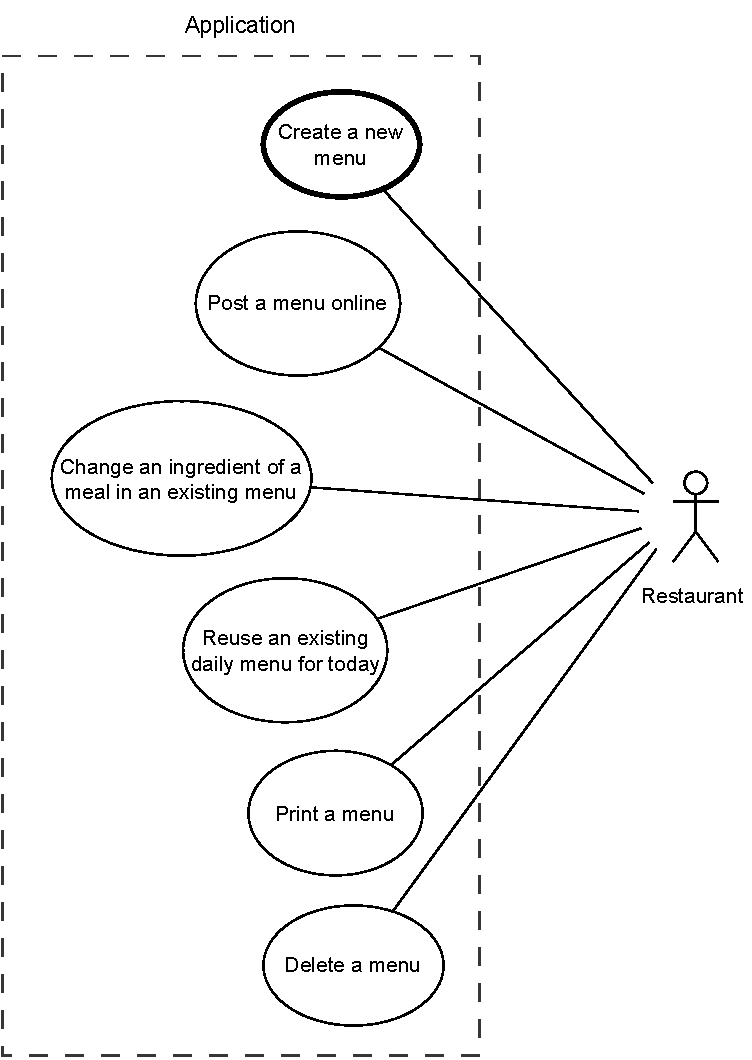
\includegraphics[width=0.62\linewidth]{master-thesis/img/use_cases_restaurant_menu_management}
%   \caption{Restaurant menu creation use cases}
% \end{figure}

% \noindent \textbf{14. Use case: Specify allergens contained in an item of a menu}

% \begin{center}
%   \begin{tabular}{| l | p{10.75cm} | }
%     \hline
%     Actor        & Restaurant \\
%     \hline
%     Description  &  \\
%     \hline
%     Scenario     &
%     \begin{minipage}[t]{\linewidth}
%       \begin{enumerate}[leftmargin=*,nosep,before=\vspace{-0.575\baselineskip},after=\strut]
%         \item ...
%         \item ... \textbf{A1}
%         \item ...
%       \end{enumerate}
%     \end{minipage}
%     \\
%     \hline
%     Alternatives &
%     \begin{minipage}[t]{\linewidth}
%       \begin{description}[nosep,after=\strut]
%         \item [A1:] ...
%       \end{description}
%     \end{minipage}
%     \\
%     \hline
%   \end{tabular}
%   \newline
% \end{center}

% \noindent \textbf{15. Use case: Specify items of a menu}

% \begin{center}
%   \begin{tabular}{| l | p{10.75cm} | }
%     \hline
%     Actor        & Restaurant \\
%     \hline
%     Description  &  \\
%     \hline
%     Scenario     &
%     \begin{minipage}[t]{\linewidth}
%       \begin{enumerate}[leftmargin=*,nosep,before=\vspace{-0.575\baselineskip},after=\strut]
%         \item ...
%         \item ... \textbf{A1}
%         \item ...
%       \end{enumerate}
%     \end{minipage}
%     \\
%     \hline
%     Alternatives &
%     \begin{minipage}[t]{\linewidth}
%       \begin{description}[nosep,after=\strut]
%         \item [A1:] ...
%       \end{description}
%     \end{minipage}
%     \\
%     \hline
%   \end{tabular}
%   \newline
% \end{center}

% \noindent \textbf{16. Use case: Create a daily menu for tomorrow}

% \begin{center}
%   \begin{tabular}{| l | p{10.75cm} | }
%     \hline
%     Actor        & Restaurant \\
%     \hline
%     Scenario     &
%     \begin{minipage}[t]{\linewidth}
%       \begin{enumerate}[leftmargin=*,nosep,before=\vspace{-0.575\baselineskip},after=\strut]
%         \item The restaurant employee logs in to the application.
%         \item The restaurant employee clicks a button labeled "Create new menu".
%         \item The application asks the restaurant employee what kind of menu they would like to create.
%         \item The restaurant employee chooses that they wish to create a daily menu.
%         \item The application asks the restaurant employee whether they want to use an existing menu as a template.
%         \item The restaurant employee denies by clicking a "No, create a new menu" button.
%         \item The restaurant employee specifies items of the menu.
%         \item The restaurant employee specifies which day the menu will be valid.
%         \item The restaurant employee clicks a "Save menu" button.
%         \item The application saves the menu.
%       \end{enumerate}
%     \end{minipage}
%     \\
%     \hline
%     % Alternatives &
%     % \begin{minipage}[t]{\linewidth}
%     %   \begin{description}[nosep,after=\strut]
%     %     \item [A1:] ...
%     %   \end{description}
%     % \end{minipage}
%     % \\
%     % \hline
%   \end{tabular}
%   \newline
% \end{center}

% \noindent \textbf{17. Use case: Specify allergens contained in a meal}

% \begin{center}
%   \begin{tabular}{| l | p{10.75cm} | }
%     \hline
%     Actor        & Restaurant \\
%     \hline
%     Scenario     &
%     \begin{minipage}[t]{\linewidth}
%       \begin{enumerate}[leftmargin=*,nosep,before=\vspace{-0.575\baselineskip},after=\strut]
%         \item The restaurant employee logs in to the application.
%         \item The restaurant employee clicks a "Create a menu" button.
%         \item The application asks the restaurant employee what kind of menu they would like to create.
%         \item The restaurant employee selects one of the options.
%         \item The restaurant employee clicks a plus sign on the new menu to add an item to it.
%         \item The restaurant employee adds information about the food item.
%         \item The application gives the restaurant employee a list of all allergens. \textbf{A1}
%         \item The restaurant employee selects allergens which are contained in the meal.
%         \item The restaurant employee clicks a "Save menu" button.
%         \item The application saves the menu.
%       \end{enumerate}
%     \end{minipage}
%     \\
%     \hline
%     Alternatives &
%     \begin{minipage}[t]{\linewidth}
%       \begin{description}[nosep,after=\strut]
%         \item [A1:] The restaurant employee starts typing the name of an ingredient. The application provides predefined ingredients and automatically adds allergens contained in the selected ingredient as the food item's allergens. The restaurant employee then continues with step 9.
%       \end{description}
%     \end{minipage}
%     \\
%     \hline
%   \end{tabular}
%   \newline
% \end{center}

% \noindent \textbf{18. Use case: Create a daily menu which will repeat each Tuesday}

% \begin{center}
%   \begin{tabular}{| l | p{10.75cm} | }
%     \hline
%     Actor        & Restaurant \\
%     \hline
%     Description  &  \\
%     \hline
%     Scenario     &
%     \begin{minipage}[t]{\linewidth}
%       \begin{enumerate}[leftmargin=*,nosep,before=\vspace{-0.575\baselineskip},after=\strut]
%         \item The restaurant employee logs in to the application.
%         \item The restaurant employee clicks a button labeled "Create new menu". 
%         \item The application asks the restaurant employee what kind of menu they would like to create.
%         \item The restaurant employee chooses that they wish to create a daily menu.
%         \item The application asks the restaurant employee whether they want to use an existing menu as a template.
%         \item The restaurant employee denies by clicking a "No, create a new menu" button.
%         \item The restaurant employee specifies items of the menu.
%         \item The restaurant employee specifies that the menu will be valid the next Tuesday.
%         \item The restaurant employee ensures that a checkbox labeled "Repeat every week" is checked.
%         \item The restaurant employee clicks a "Save menu" button.
%         \item The application saves the menu.
%       \end{enumerate}
%     \end{minipage}
%     \\
%     \hline
%     % Alternatives &
%     % \begin{minipage}[t]{\linewidth}
%     %   \begin{description}[nosep,after=\strut]
%     %     \item [A1:] 
%     %   \end{description}
%     % \end{minipage}
%     % \\
%     % \hline
%   \end{tabular}
%   \newline
% \end{center}

% \noindent \textbf{19. Use case: Create a stable menu}

% \begin{center}
%   \begin{tabular}{| l | p{10.75cm} | }
%     \hline
%     Actor        & Restaurant \\
%     \hline
%     Description  & A restaurant's management wants its restaurant to have a stable menu which will be valid every day. \\
%     \hline
%     Scenario     &
%     \begin{minipage}[t]{\linewidth}
%       \begin{enumerate}[leftmargin=*,nosep,before=\vspace{-0.575\baselineskip},after=\strut]
%         \item The restaurant employee logs in to the application.
%         \item The restaurant employee clicks a button labeled "Create new menu". 
%         \item The application asks the restaurant employee what kind of menu they would like to create.
%         \item The restaurant employee chooses that they wish to create a stable menu.
%         \item The restaurant employee specifies items of the menu.
%         \item The restaurant employee clicks a "Save menu" button.
%         \item The application saves the menu.
%       \end{enumerate}
%     \end{minipage}
%     \\
%     \hline
%     % Alternatives &
%     % \begin{minipage}[t]{\linewidth}
%     %   \begin{description}[nosep,after=\strut]
%     %     \item [A1:] ...
%     %   \end{description}
%     % \end{minipage}
%     % \\
%     % \hline
%   \end{tabular}
%   \newline
% \end{center}

% \noindent \textbf{20. Use case: Create daily menus for the next week}

% \begin{center}
%   \begin{tabular}{| l | p{10.75cm} | }
%     \hline
%     Actor        & Restaurant \\
%     \hline
%     Description  &  \\
%     \hline
%     Scenario     &
%     \begin{minipage}[t]{\linewidth}
%       \begin{enumerate}[leftmargin=*,nosep,before=\vspace{-0.575\baselineskip},after=\strut]
%         \item The restaurant employee logs in to the application.
%         \item The restaurant employee clicks a button labeled "Create new menu".
%         \item The application asks the restaurant employee what kind of menu they would like to create.
%         \item The restaurant employee chooses that they wish to create a daily menu.
%         \item The restaurant employee specifies items of the menu.
%         \item The restaurant employee specifies which day the menu will be valid.
%         \item The restaurant employee clicks a "Save menu" button.
%         \item The application saves the menu.
%         \item The restaurant employee begins again with step 2 until menus for the whole week are created.
%       \end{enumerate}
%     \end{minipage}
%     \\
%     \hline
%     % Alternatives &
%     % \begin{minipage}[t]{\linewidth}
%     %   \begin{description}[nosep,after=\strut]
%     %     \item [A1:] ...
%     %   \end{description}
%     % \end{minipage}
%     % \\
%     % \hline
%   \end{tabular}
%   \newline
% \end{center}

% \noindent \textbf{21. Use case: Create a list of beverages}

% \begin{center}
%   \begin{tabular}{| l | p{10.75cm} | }
%     \hline
%     Actor        & Restaurant \\
%     \hline
%     Description  &  \\
%     \hline
%     Scenario     &
%     \begin{minipage}[t]{\linewidth}
%       \begin{enumerate}[leftmargin=*,nosep,before=\vspace{-0.575\baselineskip},after=\strut]
%         \item The restaurant employee logs in to the application.
%         \item The restaurant employee clicks a button labeled "Create new menu". 
%         \item The application asks the restaurant employee what kind of menu they would like to create.
%         \item The restaurant employee chooses that they wish to create a list of beverages.
%         \item The restaurant employee specifies beverages of the menu.
%         \item The restaurant employee clicks a "Save menu" button.
%         \item The application saves the menu.
%       \end{enumerate}
%     \end{minipage}
%     \\
%     \hline
%     % Alternatives &
%     % \begin{minipage}[t]{\linewidth}
%     %   \begin{description}[nosep,after=\strut]
%     %     \item [A1:] ...
%     %   \end{description}
%     % \end{minipage}
%     % \\
%     % \hline
%   \end{tabular}
%   \newline
% \end{center}

% \noindent \textbf{22. Use case: Create a stable menu in a foreign language}

% \begin{center}
%   \begin{tabular}{| l | p{10.75cm} | }
%     \hline
%     Actor        & Restaurant \\
%     \hline
%     Description  & A restaurant's management wishes to have \\
%     \hline
%     Scenario     &
%     \begin{minipage}[t]{\linewidth}
%       \begin{enumerate}[leftmargin=*,nosep,before=\vspace{-0.575\baselineskip},after=\strut]
%         \item The restaurant employee logs in to the application.
%         \item The restaurant employee clicks a button labeled "Create new menu". 
%         \item The application asks the restaurant employee what kind of menu they would like to create.
%         \item The restaurant employee selects that they wish to create a stable menu.

%         \item The restaurant employee selects what currency to use in the menu.
%         \item The restaurant employee selects what weight measurement units to use in the menu.

%         \item The restaurant employee clicks a button labeled "Add category".
%         \item The application displays a screen for adding a new category.
%         \item The restaurant employee specifies the name of a new category of the menu in the foreign language.
%         \item The restaurant employee clicks an "Add" button.
%         \item The application adds the category to the menu.
%         \item The restaurant employee repeats steps x to y until they have created all categories of the new menu.
        
%         \item The restaurant employee clicks an "Add item" button.
%         \item The application asks the restaurant employee whether they would like to add a meal or a drink to the menu.
%         \item The restaurant employee selects that they wish to add a meal to the menu. A1 drink
%         \item The application displays a screen for adding a new meal to the menu.
%         \item The restaurant employee specifies the meal's name in the foreign language.
%         \item The restaurant employee specifies the meal's price and weight.
%         \item The restaurant employee clicks a button labeled "Add ingredient".
%         \item The application provides a list of possible ingredients.
%         \item The restaurant employee selects an ingredient from the list and clicks "Add".
%         \item The restaurant employee repeats steps x to y until all ingredients of the meal are added.
%         \item The restaurant employee clicks a button labeled "Add allergen". A2 - the application fills allergens contained in the ingredient automatically based on the provided ingredient
%         \item The application provides a list of possible allergens.
%         \item The restaurant employee selects an allergen from the list and clicks "Add".
%         \item The restaurant employee repeats steps x to y until all allergens of the meal are specified.
%         \item The restaurant employee repeats steps x to y until they have specified all items of the menu.

%         \item The restaurant employee clicks a "Save menu" button.
%         \item The application saves the menu.
%       \end{enumerate}
%     \end{minipage}
%     \\
%     \hline
%     Alternatives &
%     \begin{minipage}[t]{\linewidth}
%       \begin{description}[nosep,after=\strut]
%         \item [A1:] ...
%       \end{description}
%     \end{minipage}
%     \\
%     \hline
%   \end{tabular}
%   \newline
% \end{center}

% \noindent \textbf{x. Use case: Create a new menu}

% \begin{center}
%   \begin{tabular}{| l | p{10.75cm} | }
%     \hline
%     Actor        & Restaurant \\
%     \hline
%     Scenario     &
%     \begin{minipage}[t]{\linewidth}
%       \begin{enumerate}[leftmargin=*,nosep,before=\vspace{-0.575\baselineskip},after=\strut]
%         \item The restaurant employee clicks a button labeled "Create new menu". 
%         \item The application displays a screen for creating a new menu.
%         \item The restaurant employee creates categories of the new menu. \textbf{A1}
%         \item The restaurant employee specifies items, along with allergens contained in them, and assign them to the categories of the new menu.
%         \item The restaurant employee clicks a "Save" button and the application saves the menu.
%       \end{enumerate}
%     \end{minipage}
%     \\
%     \hline
%     Alternatives &
%     \begin{minipage}[t]{\linewidth}
%       \begin{description}[nosep,after=\strut]
%         \item [A1:] The restaurant employee skips the creation of categories and only specifies the items of the menu. The restaurant employee then continues with step 5.
%       \end{description}
%     \end{minipage}
%     \\
%     \hline
%   \end{tabular}
%   \newline
% \end{center}

% \noindent \textbf{x. Use case: Select what currency to use in a menu}

% \begin{center}
%   \begin{tabular}{| l | p{10.75cm} | }
%     \hline
%     Actor        & Restaurant \\
%     \hline
%     Description  & A restaurant employee has created an empty menu and wants to set what currency to use in a menu. \\
%     \hline
%     Scenario     &
%     \begin{minipage}[t]{\linewidth}
%       \begin{enumerate}[leftmargin=*,nosep,before=\vspace{-0.575\baselineskip},after=\strut]
%         \item The restaurant employee clicks a button labeled "Choose currency for the menu".
%         \item The application provides a predefined list of currencies. 
%         \item The restaurant employee selects the desired currency and clicks an "Ok" button.
%         \item The application sets the selected currency for the menu.
%       \end{enumerate}
%     \end{minipage}
%     \\
%     \hline
%   \end{tabular}
%   \newline
% \end{center}

% \noindent \textbf{x. Use case: Select what weight units to use in a menu}

% \begin{center}
%   \begin{tabular}{| l | p{10.75cm} | }
%     \hline
%     Actor        & Restaurant \\
%     \hline
%     Description  & A restaurant employee has created an empty menu and wants to set what weight units to use in it. \\
%     \hline
%     Scenario     &
%     \begin{minipage}[t]{\linewidth}
%       \begin{enumerate}[leftmargin=*,nosep,before=\vspace{-0.575\baselineskip},after=\strut]
%         \item The restaurant employee clicks a button labeled "Choose weight units".
%         \item The application provides a predefined set of weight units.
%         \item The restaurant employee selects the desired weight unit and clicks an "Ok" button.
%         \item The application sets the selected weight unit for the menu.
%       \end{enumerate}
%     \end{minipage}
%     \\
%     \hline
%   \end{tabular}
%   \newline
% \end{center}

% \noindent \textbf{x. Use case: Add a category to a menu}

% \begin{center}
%   \begin{tabular}{| l | p{10.75cm} | }
%     \hline
%     Actor        & Restaurant \\
%     \hline
%     Description  & A restaurant employee has created an empty menu and wants to add a category to it. \\
%     \hline
%     Scenario     &
%     \begin{minipage}[t]{\linewidth}
%       \begin{enumerate}[leftmargin=*,nosep,before=\vspace{-0.575\baselineskip},after=\strut]
%         \item The restaurant employee clicks a button labeled "Add category".
%         \item The restaurant employee specifies the name of the category.
%         \item The application adds the category to the menu.
%       \end{enumerate}
%     \end{minipage}
%     \\
%     \hline
%   \end{tabular}
%   \newline
% \end{center}

% \noindent \textbf{x. Use case: Specify allergens contained in an item of a menu}

% \begin{center}
%   \begin{tabular}{| l | p{10.75cm} | }
%     \hline
%     Actor        & Restaurant \\
%     \hline
%     Description  & A restaurant's employee is creating a menu. They have added an item to the menu and want to specify allergens contained in it. \\
%     \hline
%     Scenario     &
%     \begin{minipage}[t]{\linewidth}
%       \begin{enumerate}[leftmargin=*,nosep,before=\vspace{-0.575\baselineskip},after=\strut]
%         \item The restaurant employee clicks a button labeled "Add allergen". \textbf{A1}
%         \item The application provides a predefined list of possible allergens.
%         \item The restaurant employee selects an allergen from the list and clicks "Add".
%         \item The restaurant employee repeats steps x to y until all allergens of the item are added.
%       \end{enumerate}
%     \end{minipage}
%     \\
%     \hline
%     Alternatives &
%     \begin{minipage}[t]{\linewidth}
%       \begin{description}[nosep,after=\strut]
%         \item [A1:] The application adds allergens contained in the ingredient automatically based on the provided ingredient (see x. Use case: Add an item to a menu).
%       \end{description}
%     \end{minipage}
%     \\
%     \hline
%   \end{tabular}
%   \newline
% \end{center}

% \noindent \textbf{x. Use case: Add an item to a menu}

% \begin{center}
%   \begin{tabular}{| l | p{10.75cm} | }
%     \hline
%     Actor        & Restaurant \\
%     \hline
%     Description  & A restaurant's employee has created an empty menu and wants to add an item to it. \\
%     \hline
%     Scenario     &
%     \begin{minipage}[t]{\linewidth}
%       \begin{enumerate}[leftmargin=*,nosep,before=\vspace{-0.575\baselineskip},after=\strut]
%         \item The restaurant employee clicks an "Add item" button.
%         \item The application displays a screen for adding an item to a menu.
%         \item The restaurant employee specifies the item's name, price and amount.
%         \item The restaurant employee clicks a button labeled "Add ingredient".
%         \item The application provides a predefined list of ingredients.
%         \item The restaurant employee selects an ingredient from the list and clicks "Add". \textbf{A1}
%         \item The restaurant employee repeats steps x to y until all ingredients of the item are added.
%         \item The restaurant employee adds allergens contained in the item (see x. Use case: Specify allergens contained in an item of a menu).
%       \end{enumerate}
%     \end{minipage}
%     \\
%     \hline
%     Alternatives &
%     \begin{minipage}[t]{\linewidth}
%       \begin{description}[nosep,after=\strut]
%         \item [A1:] The restaurant employee also specifies the amount of the ingredient contained in the item. The restaurant employee continues with step x.
%       \end{description}
%     \end{minipage}
%     \\
%     \hline
%   \end{tabular}
%   \newline
% \end{center}

% \noindent \textbf{x. Use case: Add my restaurant's information to a menu}

% \begin{center}
%   \begin{tabular}{| l | p{10.75cm} | }
%     \hline
%     Actor        & Restaurant \\
%     \hline
%     Description  & A restaurant's employee has created an empty menu and wants to add basic information about the restaurant. \\
%     \hline
%     Scenario     &
%     \begin{minipage}[t]{\linewidth}
%       \begin{enumerate}[leftmargin=*,nosep,before=\vspace{-0.575\baselineskip},after=\strut]
%         \item The restaurant employee clicks a button labeled "Add restaurant information".
%         \item The application displays a screen for adding basic restaurant information.
%         \item The restaurant employee specifies the restaurant's name, address and phone number.
%         \item The restaurant employee clicks an "Add" button.
%         \item The application adds the specified information to the menu. 
%       \end{enumerate}
%     \end{minipage}
%     \\
%     \hline
%   \end{tabular}
%   \newline
% \end{center}

% \noindent \textbf{x. Use case: Specify where should the application store my data }

% \begin{center}
%   \begin{tabular}{| l | p{10.75cm} | }
%     \hline
%     Actor        & Restaurant \\
%     \hline
%     Description  &  \\
%     \hline
%     Scenario     &
%     \begin{minipage}[t]{\linewidth}
%       \begin{enumerate}[leftmargin=*,nosep,before=\vspace{-0.575\baselineskip},after=\strut]
%         \item ...
%         \item ... \textbf{A1}
%         \item ...
%       \end{enumerate}
%     \end{minipage}
%     \\
%     \hline
%     Alternatives &
%     \begin{minipage}[t]{\linewidth}
%       \begin{description}[nosep,after=\strut]
%         \item [A1:] ...
%       \end{description}
%     \end{minipage}
%     \\
%     \hline
%   \end{tabular}
%   \newline
% \end{center}
\section{User requirements}
It is good practice to use language consistently throughout requirements and that is why we are going to resolve what keywords will we use and what will they mean.
If a requirement states that the application \textbf{shall} do something then it means that the requirement is mandatory for the application and has to be addressed in the design phase which follows after this chapter. 
The word \textbf{should} is used in requirements which are desired by users but are not critical for the application's usability.
Last but not least, usage of the word \textbf{must} indicates a domain constraint.
Also, we will substitute the user role restaurant for \emph{restaurant employee} where it will be more convenient.

\subsection{Functional requirements}
\subsubsection{Guest user role requirements}
A guest is expected to be logged in to the application if not stated otherwise in a requirement.

\begin{description}
    \item [Req. 1.1:] The application shall enable a restaurant guest to specify what allergies they have.
    \item [Req. 1.2:] The application shall enable a restaurant guest to specify what diets they are on.
    \item [Req. 1.3:] The application should enable a restaurant guest to specify what food and beverages they like and dislike.
    \item [Req. 1.4:] The application shall enable a restaurant guest to view a menu of the restaurant which is personalized based on the guest's profile.

    \emph{Rationale:} A personalized menu highlights or hides items of a menu, so that a guest can quickly choose what they want to order. 
    \item [Req. 1.5:] The application shall be able to sort meals in a menu by whether a viewing guest can eat them according to their profile.
    \item [Req. 1.6:] The application shall be able to hide meals of a menu which, according to their profile, a viewing guest cannot eat.
    \item [Req. 1.7:] A guest shall be able to view a restaurant's menu by specifying its IRI.
    \item [Req. 1.8:] A guest should be able to view a menu by scanning a QR code on a printed menu.

    \emph{Rationale:} The QR code will link to the URL of the application and will provide it with the IRI of the menu just like in the requirement 1.7.
    \item [Req. 1.9:] A guest should be able to specify the IRI of a restaurant and browse its menus.

    \emph{Rationale:} A restaurant can have multiple menus valid at the same time. 
    \item [Req. 1.10:] A guest shall be able to mark a restaurant as their favorite.
    
    \emph{Rationale:} The guest should have a set of their favorite restaurants which will be used for other application's functionality like the requirement 1.11.
    \item [Req. 1.11:] A guest shall be able to view currently served meals by their favorite restaurants.
    \item [Req. 1.12:] A guest should be able to filter menu items based on what diet they are part of.
    \item [Req. 1.13:] A non-authenticated guest should have access to the application's functionalities stated in requirements 1.7, 1.8, 1.9 and 1.12. 

    \emph{Rationale:} None of these features require a guest to be logged in. The application should be also useful for people without a profile.
\end{description}

\subsubsection{Restaurant user role requirements}
\begin{description}
    \item [Req. 2.1:] A restaurant employee shall be able to create a menu for a specific day.

    \emph{Rationale:} Restaurants often have daily menus.
    \item [Req. 2.2:] A restaurant employee shall be able to create a stable menu.

    \emph{Rationale:} Most restaurants have a stable menu which is valid every day and does not change often.
    \item [Req. 2.3:] A restaurant employee should be able to create a list of beverages.

    \emph{Rationale:} Some restaurants have a separate menu for meals and for drinks.
    \item [Req. 2.4:] A restaurant employee should be able to print a menu.

    \emph{Rationale:} A printed menu can be put on tables.
    \item [Req. 2.5:] A printed menu should contain a QR code which will link a guest to the application.

    \emph{Rationale:} The QR code will provide the application with the IRI of the menu.
    \item [Req. 2.6:] The application shall enable a restaurant employee to edit a previously created menu.
    \item [Req. 2.7:] The application shall enable a restaurant employee to delete a previously created menu.
    \item [Req. 2.8:] A restaurant employee should be able to set a daily menu to repeat periodically for a certain day of the week.

    \emph{Rationale:} A daily menu can be the same for a certain day of the week.
    \item [Req. 2.9:] A restaurant employee should be able to specify categories and subcategories of a menu.

    \emph{Rationale:} A menu typically consists of categories like soups, appetizers, desserts etc. These categories can have subcategories, for instance a category "Drinks" can have subcategories "Wine" and "Non-alcoholic".
    \item [Req. 2.10:] Each item of a menu should belong to either none or exactly one category.
    \item [Req. 2.11:] A meal in a menu should contain an ID, label, price, weight or volume, ingredients and allergens.
    \item [Req. 2.12:] A restaurant employee should be able to specify weights of ingredients contained in a meal.

    \emph{Rationale:} The weight in the requirement 2.12 is the weight of a whole meal, i.e. all ingredients' weights combined.
    \item [Req. 2.13:] A menu should optionally contain a restaurant's name, address and phone number.

    \emph{Rationale:} Optionally means that the creator of a menu can decide whether to put these information on the menu or not.
    \item [Req. 2.14:] A restaurant employee should be able to use a previously created menu as the starting point for creating a new menu.

    \emph{Rationale:} A restaurant employee might want to create a new menu which differs only in some items of an existing menu.
    \item [Req. 2.15:] A restaurant employee should be able to specify what currency to use in a menu.
    \item [Req. 2.16:] A restaurant employee should be able to specify what weight and volume units to use for liquid items in a menu.
    \item [Req. 2.17:] A restaurant employee should be able to specify what font to use in a menu.
    \item [Req. 2.18:] The application should offer a few empty menus as templates for a restaurant employee to choose from when creating a menu.

    \emph{Rationale:} These templates can differ in what categories they have, what font they use or what currency and weight units they use.
    \item [Req. 2.19:] A restaurant employee should be able to set that a menu shall use allergen labels for displaying allergen information.

    \emph{Rationale:} Allergens can be listed within an item's description.
    \item [Req. 2.20:] A restaurant employee should be able to set that a menu shall use numbers for displaying allergen information.

    \emph{Rationale:} A menu item can contain numbers which represent allergens. This is more concise than using labels from the requirement x. 
\end{description}

\subsection{Non-functional requirements}
\begin{description}
    \item [Req. 3.1:] Each item of a menu must have its allergens specified.
    
    \emph{Rationale:} In the EU, there are laws\footnote{\url{https://eur-lex.europa.eu/legal-content/EN/ALL/?uri=celex\%3A32011R1169}  \label{fnlabel}} which mandate restaurants to list allergens contained in the foods they serve.
    \item [Req. 3.2:] A menu which uses allergen numbers from requirement 2.20 must contain a legend explaining which allergen each number represents.

    \emph{Rationale:} This requirement extends the requirement 3.1.
    \item [Req. 3.3:] The application should have responsive user interface and work on mobile devices as well as on desktops.
    \item [Req. 3.4:] The application should be compatible with the latest versions of all of the commonly used browsers, namely Google Chrome of version x.y, Mozilla Firefox of version x.y, Microsoft Edge of version x.y, Opera of version x.y and Safari of version x.y.
    \item [Req. 3.5:] The application shall have a user tutorial explaining its functionality for each screen defined in the design chapter.
    \item [Req. 3.6:] The application should have an English, Czech and Slovak translations.

    \emph{Rationale:} We would like for the application to be used internationally within the European Union.
    \item [Req. 3.7:] Both guests and restaurants should be able to specify which Solid pod should the application use for storing and reading their data.

    \emph{Rationale:} A guest or a restaurant can have multiple Solid pods associated with their WebID.
\end{description}

\vspace*{\fill}
% \chapter{Existing solutions}
In this chapter we will look at currently available solutions in our problem domain. 
First part of the problem domain is for restaurants to specify allergens in food.
Second part of the problem domain is for a restaurant guest to comfortably choose what they want to eat at a restaurant, given that they have an allergy or are on a diet.

Third part is 
food preferences - what I like and dislike

% \chapter{Design}

Now we will design how to implement what we have defined in the previous chapter.

\section{Title of the first subchapter of the chapter}

\section{Title of the second subchapter of the chapter}


\chapter*{Conclusion}
\addcontentsline{toc}{chapter}{Conclusion}


%%% Bibliography
%%% Bibliography (literature used as a source)
%%%
%%% We employ bibTeX to construct the bibliography. It processes
%%% citations in the text (e.g., the \cite{...} macro) and looks up
%%% relevant entries in the bibliography.bib file.
%%%
%%% The \bibliographystyle command selects, which style will be used
%%% for references from the text. The argument in curly brackets is
%%% the name of the corresponding style file (*.bst). Both styles
%%% mentioned in this template are included in LaTeX distributions.

\bibliographystyle{plainnat}    %% Author (year)
% \bibliographystyle{unsrt}     %% [number]

\renewcommand{\bibname}{Bibliography}

%%% Generate the bibliography. Beware that if you cited no works,
%%% the empty list will be omitted completely.

\bibliography{bibliography}

%%% If case you prefer to write the bibliography manually (without bibTeX),
%%% you can use the following. Please follow the ISO 690 standard and
%%% citation conventions of your field of research.

% \begin{thebibliography}{99}
%
% \bibitem{lamport94}
%   {\sc Lamport,} Leslie.
%   \emph{\LaTeX: A Document Preparation System}.
%   2nd edition.
%   Massachusetts: Addison Wesley, 1994.
%   ISBN 0-201-52983-1.
%
% \end{thebibliography}


%%% Figures used in the thesis (consider if this is needed)
\listoffigures

%%% Tables used in the thesis (consider if this is needed)
%%% In mathematical theses, it could be better to move the list of tables to the beginning of the thesis.
\listoftables

%%% Abbreviations used in the thesis, if any, including their explanation
%%% In mathematical theses, it could be better to move the list of abbreviations to the beginning of the thesis.
\chapwithtoc{List of Abbreviations}

%%% Attachments to the master thesis, if any. Each attachment must be
%%% referred to at least once from the text of the thesis. Attachments
%%% are numbered.
%%%
%%% The printed version should preferably contain attachments, which can be
%%% read (additional tables and charts, supplementary text, examples of
%%% program output, etc.). The electronic version is more suited for attachments
%%% which will likely be used in an electronic form rather than read (program
%%% source code, data files, interactive charts, etc.). Electronic attachments
%%% should be uploaded to SIS and optionally also included in the thesis on a~CD/DVD.
%%% Allowed file formats are specified in provision of the rector no. 72/2017.
\appendix
\chapter{Attachments}

\section{First Attachment}

\openright
\end{document}
